\documentclass[12pt]{article}
\usepackage[utf8]{inputenc}
\usepackage[T1]{fontenc}
\usepackage{amsmath}
\usepackage{amsfonts}
\usepackage{amssymb}
\usepackage{physics}

\usepackage[version=4]{mhchem}
\usepackage{stmaryrd}
\usepackage{graphicx}
\usepackage[export]{adjustbox}
\graphicspath{ {./images/} }
\usepackage{hyperref}
\hypersetup{colorlinks=true, linkcolor=blue, filecolor=magenta, urlcolor=cyan,}
\urlstyle{same}

\title{CH226: Nonlinear Optics }

\author{}
\date{}


%New command to display footnote whose markers will always be hidden
\let\svthefootnote\thefootnote
\newcommand\blfootnotetext[1]{%
  \let\thefootnote\relax\footnote{#1}%
  \addtocounter{footnote}{-1}%
  \let\thefootnote\svthefootnote%
}

%Overriding the \footnotetext command to hide the marker if its value is `0`
\let\svfootnotetext\footnotetext
\renewcommand\footnotetext[2][?]{%
  \if\relax#1\relax%
    \ifnum\value{footnote}=0\blfootnotetext{#2}\else\svfootnotetext{#2}\fi%
  \else%
    \if?#1\ifnum\value{footnote}=0\blfootnotetext{#2}\else\svfootnotetext{#2}\fi%
    \else\svfootnotetext[#1]{#2}\fi%
  \fi
}

\begin{document}
\maketitle
Homework \#5 (last one!) - Spring/2022, Due Tuesday May $24^{\text {nd }}$

CCE, California Institute of Technology

\section{}

The Feynman and ladder diagrams are shown below for the four independent third-order correlation functions of a two-level system (from Andrei Tokmakoff's class notes $\left.{ }^{1}\right)$.

\begin{center}
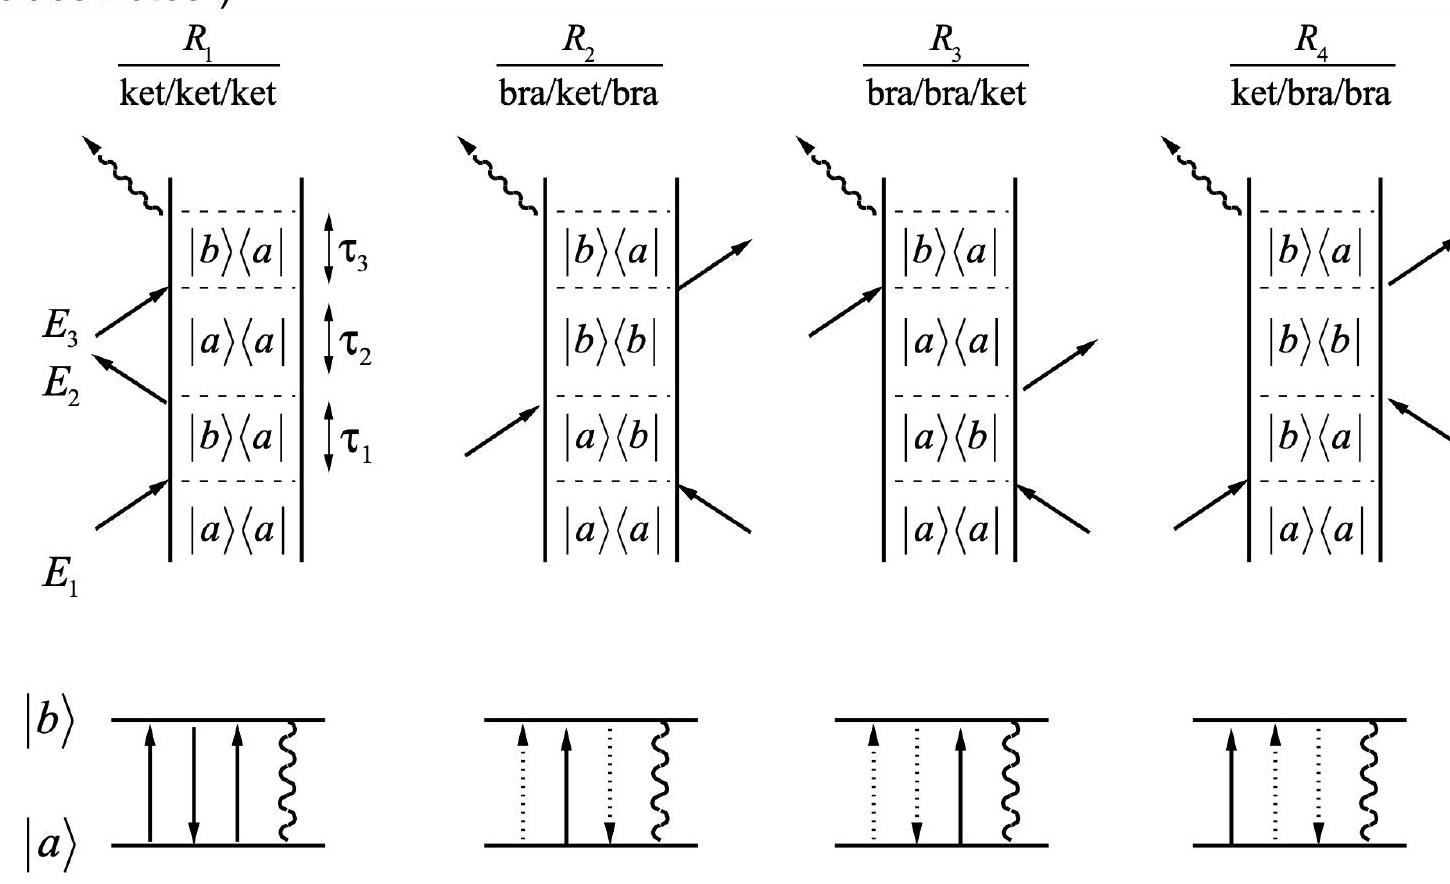
\includegraphics[max width=\textwidth]{2024_05_26_dcc5d1010257c1c9dfb7g-1}
\end{center}
\subsection{}

Verify, as quantitatively as you can, the assertion on the bottom of page $\underline{25}$, that the $R 2$ and $R 3$ diagrams depict rephasing pathways, while the R1 and R4 diagrams depict non-rephasing pathways.
\subsubsection{Answer}
Because in the R2 and R3 diagrams, during the $\tau_1$ and $\tau_3$ propagation time periods, a coherence between the ground and excited states that is created during $\tau_1$ is destroyed during $\tau_3$, and we can call it a rephasing pathway. This corresponds to acquiring a phase factor of $e^{i \omega_{ab} \tau_{1}} e^{-i \omega_{ab} \tau_{3}} = e^{i \omega_{ab}(\tau_{1}-\tau_{3})}$, so we can see the phase acquired during the first time being destroyed during the third time.\\
 In contrast, in the R1 and R4 diagrams, the coherence between the ground and excited states that is created during $\tau_1$ is added to during $\tau_3$, and so we can call it a non-rephasing pathway. This corresponds to acquiring a phase factor of $e^{i \omega_{ab} \tau_{1}} e^{i \omega_{ab} \tau_{3}} = e^{i \omega_{ab}(\tau_{1}+\tau_{3})}$, so we can see the phase acquired during the first time being added constructively during the third time.
\subsection{}
What is the expression of $\mathrm{k}_{\text {sig }}$ and $\omega_{\text {sig }}$ for each of the four diagrams? Include how you obtained these expressions.
\subsubsection{Answer}
\begin{figure}[h]
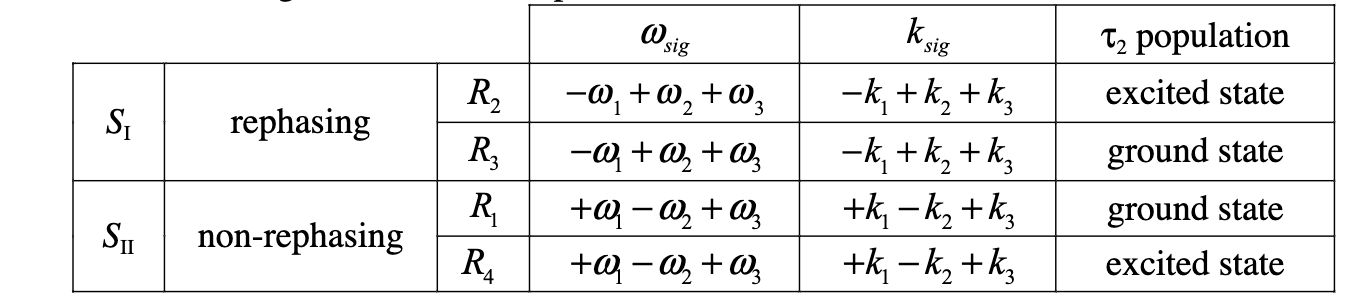
\includegraphics[max width=\textwidth, center]{table.png}
\caption{Table of the expressions for $\mathrm{k}_{\text {sig }}$ and $\omega_{\text {sig }}$ for each of the four diagrams.}
\label{fig:table}
\end{figure}
As can be seen in figure \ref{fig:table}, the sign of the angular frequency $\omega$ is always the same as that of the wave vector $k$. This is because they are connected to the energy and momentum, respectively, of the same beam. When light interacts with the ket side, we always get a positive sign for a transition from the ground to excited state, and vice versa. Because we defined the bra state as the complex conjugate of the ket state, a ground to excited state transition will correspond to a negative sign and vice versa. Application of the rules just described for the different diagrams gives the expressions in the table.
\section{}
In the diagram below, a feature in a two-dimensional nonlinear vibronic spectrum is displayed, along with the linear absorption features present in the spectrum. As quantitatively as possible, describe why the extent of inhomogeneous broadening is measured 'along the diagonal' in the $\omega_{\text {probe }} / \omega_{\text {pump }}$ plot, while dephasing is measured along the orthogonal direction.
\subsubsection{Answer}
For the inhomogeneous broadening, we are merely measuring the distribution of the transition frequencies of the molecules in the sample. So, we have a certain $\omega_{\text {pump }}$ frequency which will correspond to a transition in a particular molecular environment, but because we have many such environments within the sample, we can have a spread in frequencies of $\omega_{\text {pump }}$ that will correspond to a similar $\omega_{\text {probe }}$ frequency. In the linear plot, we see that there are many different transition frequencies due to different molecular environments and this contributes to the broadening $\Delta$. So in essence, we are measuring the section where $\omega_{\text {probe }} = \omega_{\text {pump }}$, which corresponds to the diagonal of the 2D plot. We measure the dephasing along the orthogonal direction because we are interested in one certain $\omega_{\text {pump }}$ frequency and we want to see how dephasing within the same molecules within the sample results in different $\omega_{\text {probe }}$ frequencies. In the linear plot describing the dephasing $\Gamma $, we see that for a given probe frequency, we see a large vertical spread in the signal observed. These are due to the different phases that can be acquired in a sample at a certain pump frequency.



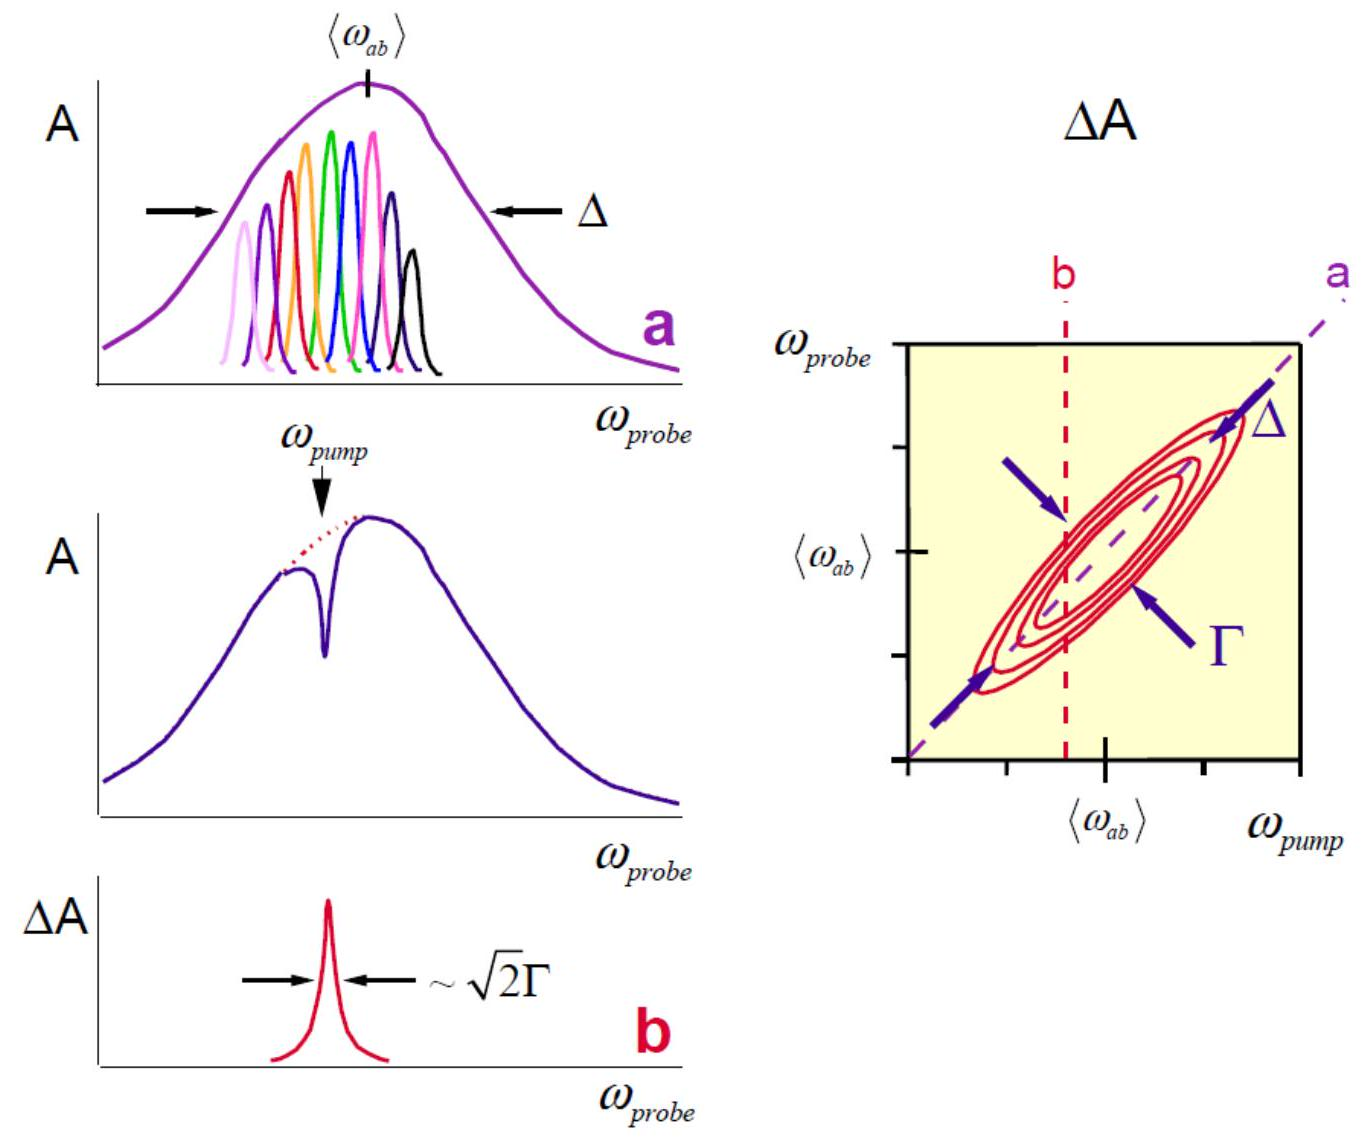
\includegraphics[max width=\textwidth, center]{2024_05_26_dcc5d1010257c1c9dfb7g-2}\\
\section{}
$2 \mathrm{D}$ electronic spectroscopy (2DES) uses pulse sequences in the visible spectral range to excite and probe electronic states.
\subsection{}

Draw a three-level energy diagram (that is, a ground state and two excited electronic states) and sketch the resulting 2DES plot that you'd expect to observe.

Label and describe any relevant features, including inhomogeneous/homogeneous broadening, excited state absorption, and from which electronic transition/coupling features arise.
\begin{figure}
  \centering
  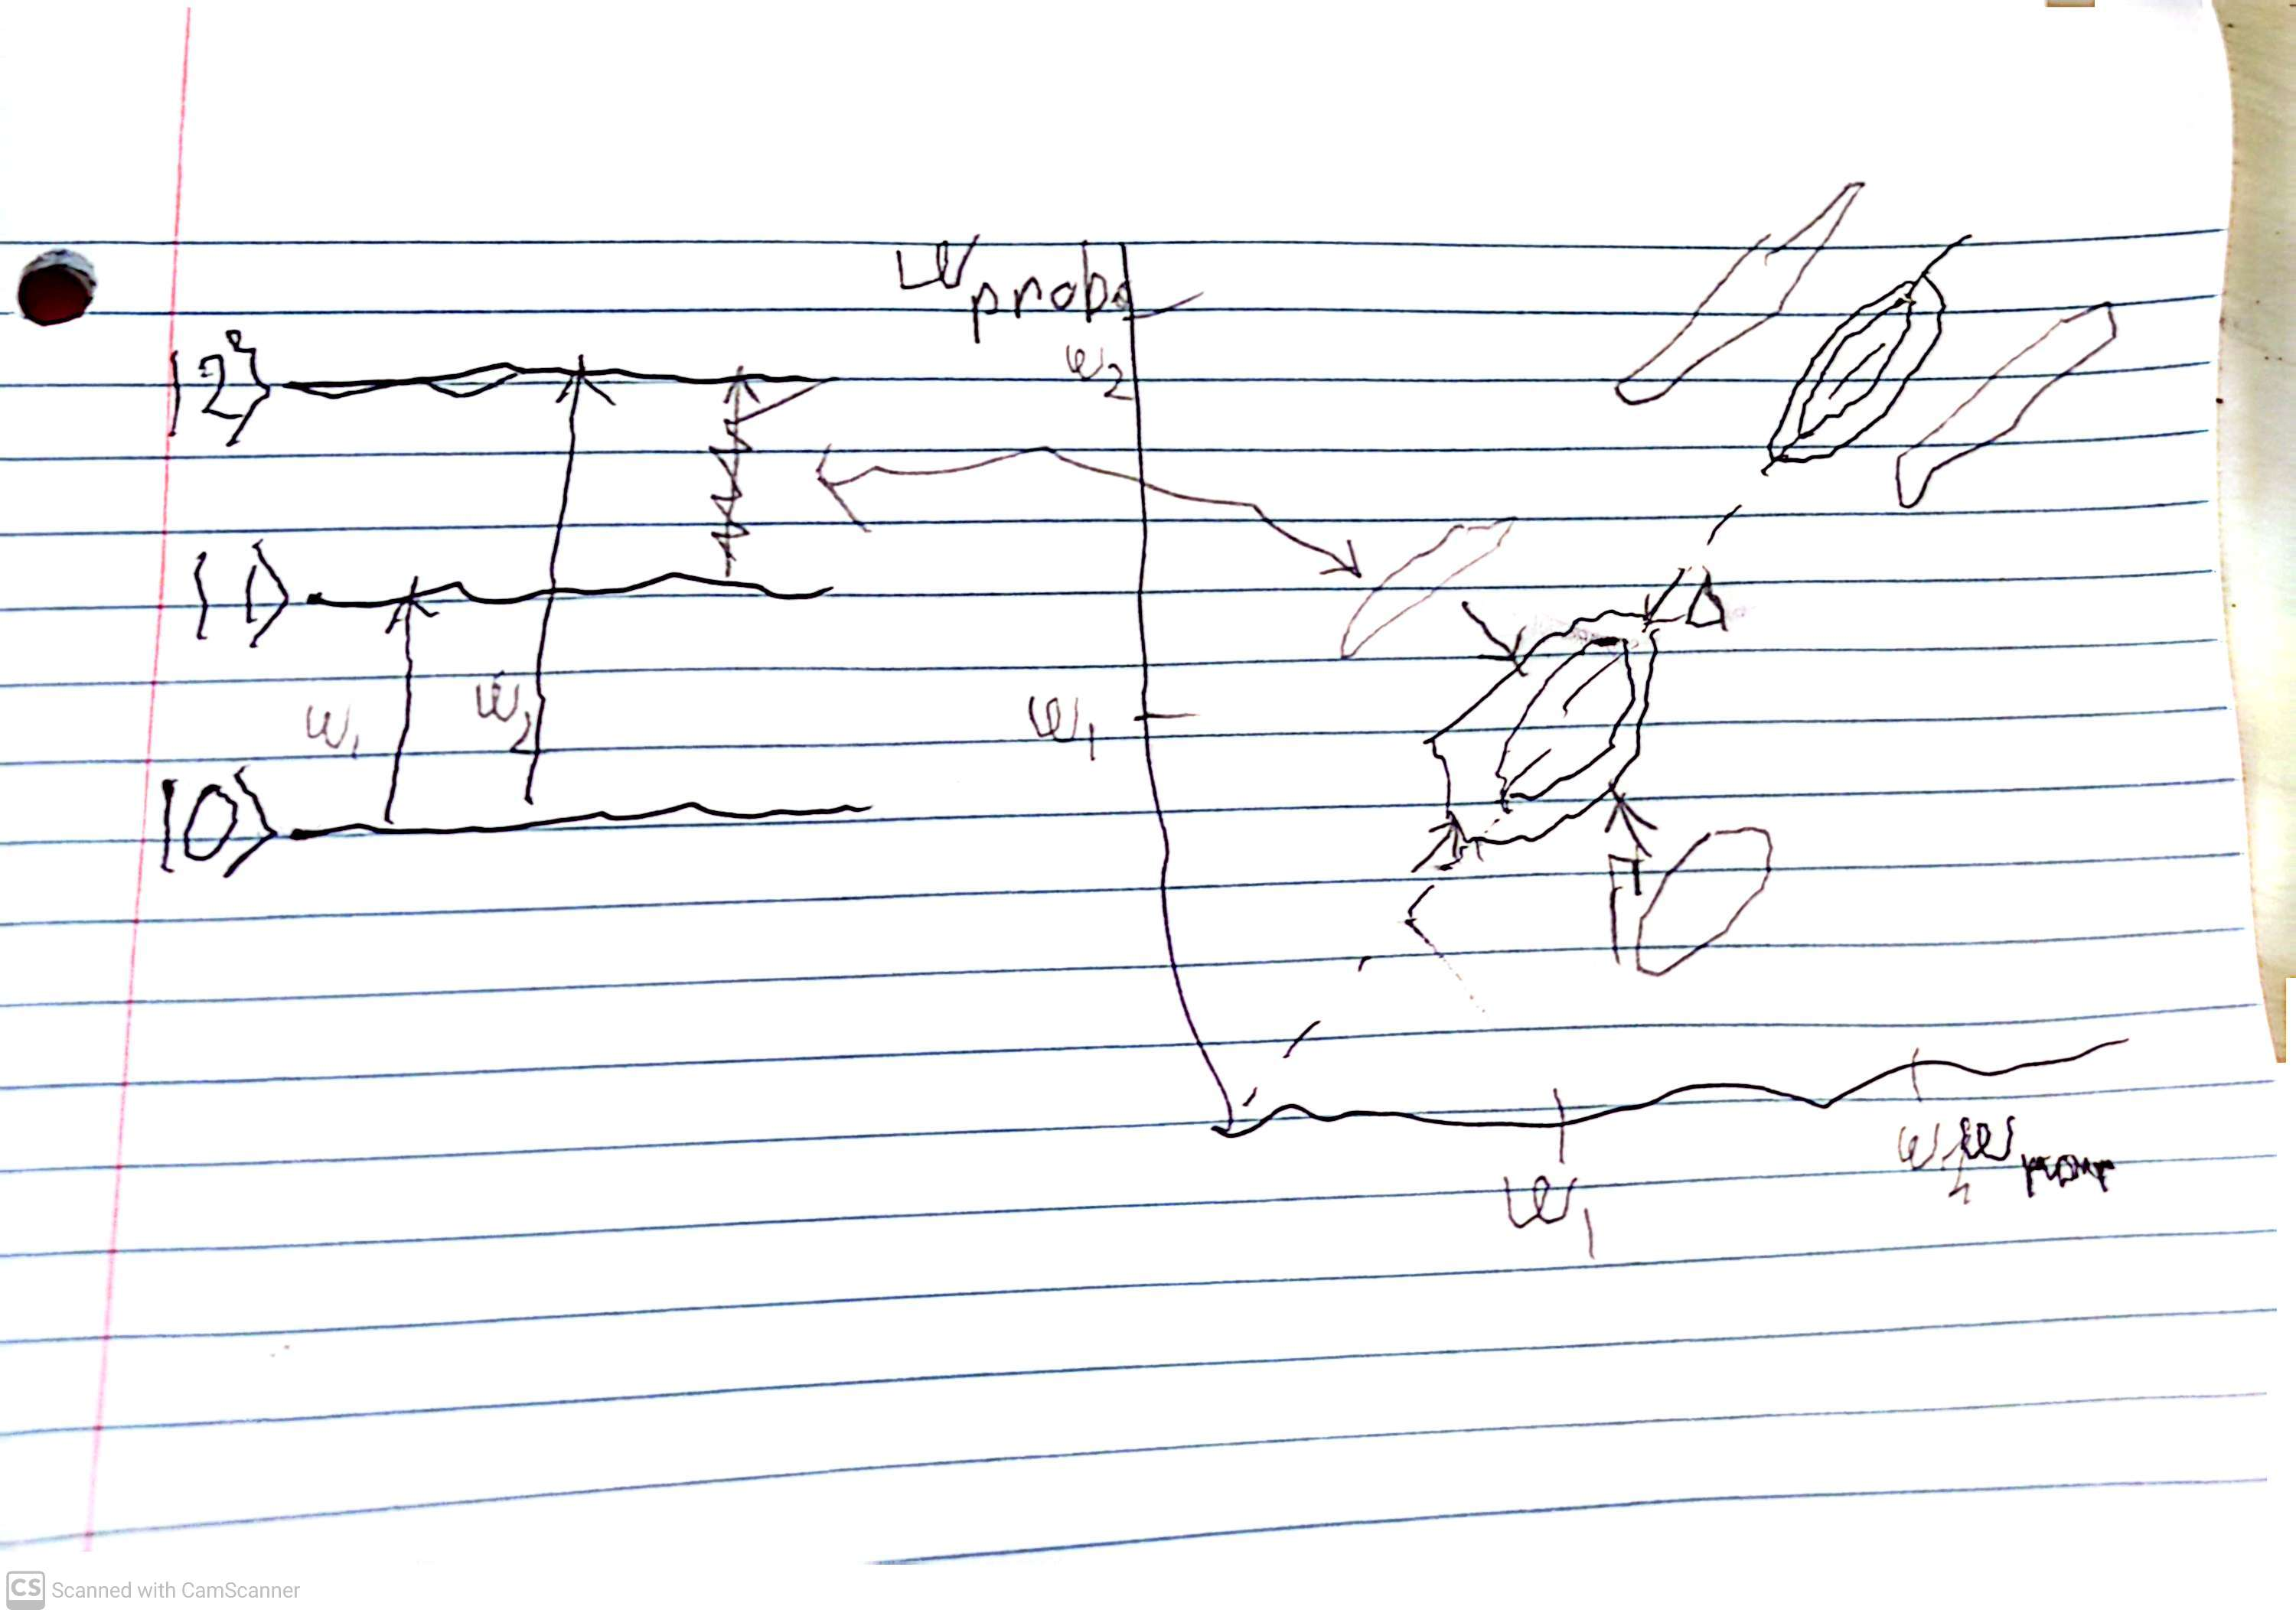
\includegraphics[max width=\textwidth]{CamScanner 05-28-2024 22.17.jpg}
  \caption{Three-level energy diagram and the resulting 2DES plot}
  \label{fig:my_label}
\end{figure}
\subsubsection{Answer}
The features that can be observed from the diagonal correspond to the $\ket{0}$ to $\ket{1}$ ($\omega _{1}$) and $\ket{2}$ ($\omega _{2}$) transitions. The inhomogeneous broadening is observed as the diagonal spread of a certain feature, and is marked by its magnitude $\Delta $. The homogeneous broadening for a certain feature is measured by the width of the feature orthogonal to the diagonal and is marked by its magnitude $\Gamma $. Since we have two different excited states, we observe two excited state absorption features at two different frequencies $\omega _{1}$ and $\omega _{2}$ along the diagonal. The coupling features can arise, marked by the ellipses off the diagonal, when a certain pump frequency is met by a different probe frequency; This can be interpreted that $\omega _{pump}$ near the frequency where it excites from the ground state to the first excited state could also correspond to an excitation from the first to the second excited state, marked by a jagged arrow on the diagram, that could be probed as well.


\end{document}